\chapter{Cromatografía}\label{ch:b2:chromatography}

Una gota de una bebida energética, diluida y filtrada, se inyecta en un tubo de acero no más largo que un bolígrafo y
relleno de granos de sílice de unos pocos micrómetros. Unos minutos después, un detector ha trazado una línea
con un puñado de picos, y a partir del área de uno de ellos el laboratorio informa de cuánta cafeína contiene la
lata, con una precisión de unos pocos por ciento. La \omterm{def:b2:chromatography:principle}{cromatografía} separa los componentes de una mezcla haciéndolos
recorrer una columna a velocidades distintas; este capítulo explica por qué viajan a velocidades distintas,
por qué sus picos tienen la anchura que tienen, cómo separar dos vecinos y cómo convertir un pico en
una cantidad.

\begin{omfigure}
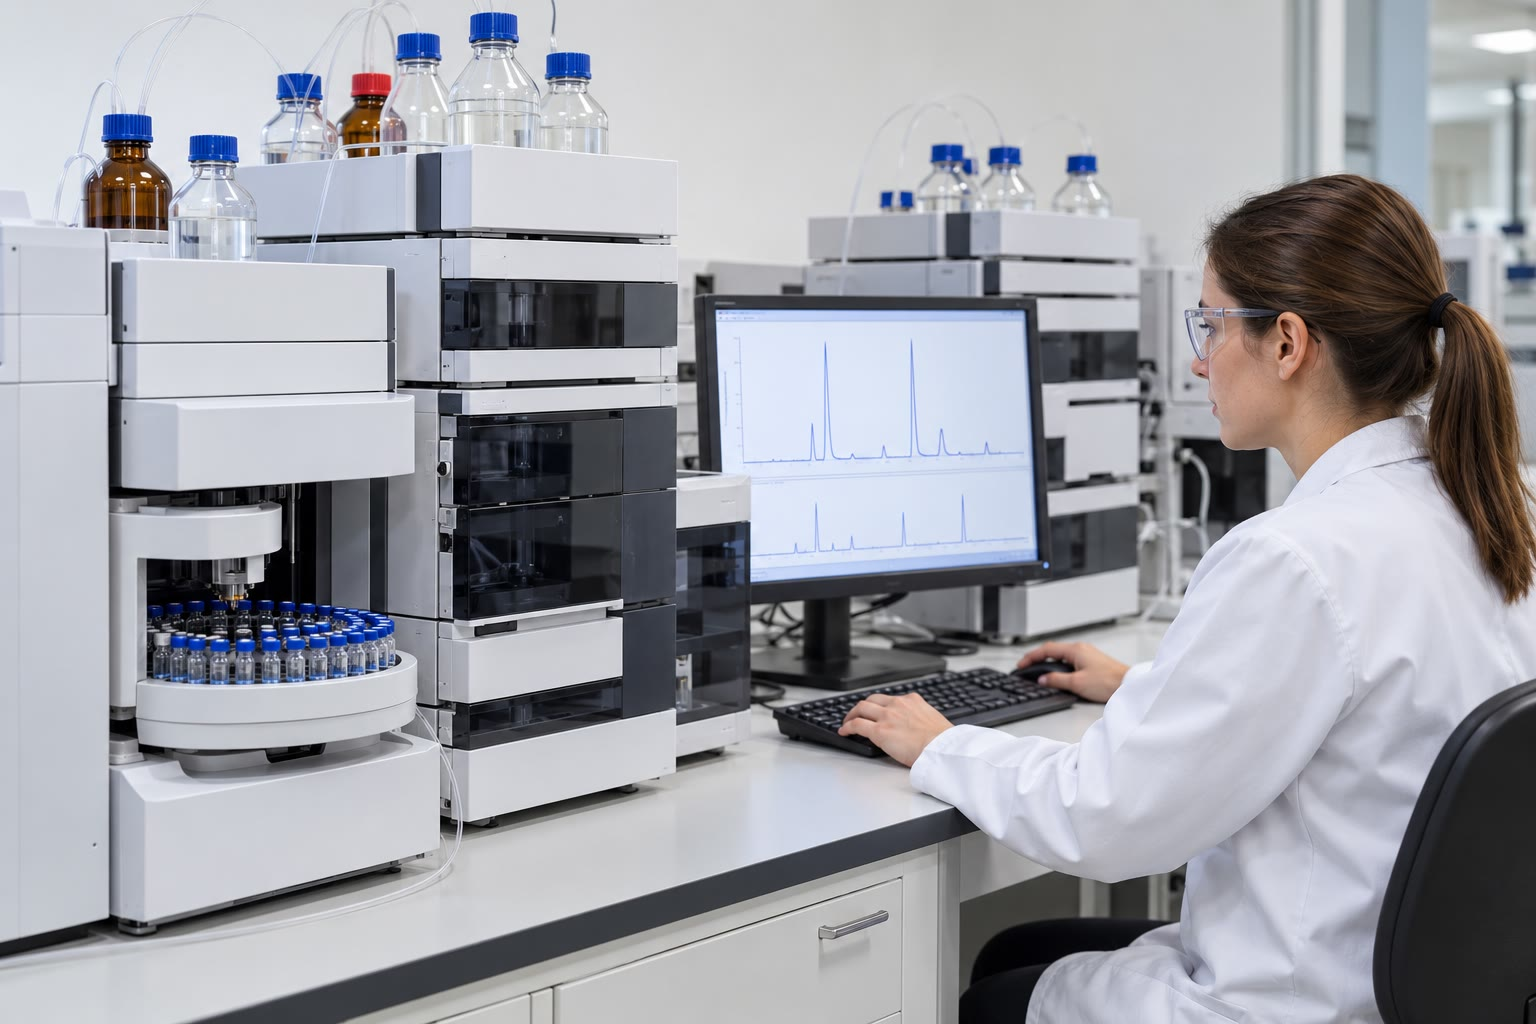
\includegraphics[width=0.58\linewidth]{images/book3/ai/b2-31-analytical-lab.jpg}

{\small Un laboratorio de análisis: cromatógrafos de líquidos con sus botellas de disolvente y una bandeja de
inyector automático con viales; los cromatogramas aparecen en la pantalla (ilustración).}
\end{omfigure}

\begin{recall}
El volumen escolar: \omterm{def:b2:chromatography:principle}{cromatografía} en papel y en capa fina, cromatograma, eluyente. El volumen del primer año: el
coeficiente de reparto, la extracción líquido--líquido, el factor de retención $R_f$ de una placa de capa fina.
\Cref{ch:b2:liquid-vapour-diagrams}: el \omterm{def:b2:liquid-vapour-diagrams:fractional-distillation}{plato teórico} de una columna de destilación.
\end{recall}

\section{Principio}

\begin{definition}[Cromatografía]\label{def:b2:chromatography:principle}
La \emph{cromatografía}\index{cromatografia@cromatografía} separa los componentes de una mezcla repartiéndolos
entre una \emph{fase estacionaria}\index{fase estacionaria}, fija en una columna o sobre una placa, y una
\emph{fase móvil}\index{fase movil@fase móvil}, un gas o un líquido que fluye a lo largo de ella. Arrastrar los componentes
a través de la columna y fuera de ella con la fase móvil es la \emph{elución}\index{elucion@elución}.
\end{definition}

Una molécula solo avanza mientras está en la \omterm{def:b2:chromatography:principle}{fase móvil}; mientras la retiene la \omterm{def:b2:chromatography:principle}{fase estacionaria},
espera. Cambia de una fase a otra millones de veces en su recorrido, de modo que su velocidad media la fija
la fracción de tiempo que pasa en cada una, es decir, su equilibrio de reparto.

\begin{definition}[Retención]\label{def:b2:chromatography:retention}
El \emph{tiempo de retención}\index{tiempo de retencion@tiempo de retención} $t_R$ de un compuesto es el tiempo que va de la inyección al
máximo de su pico; el \emph{tiempo muerto}\index{tiempo muerto} $t_M$ es el tiempo de retención de un
compuesto no retenido, que nunca entra en la \omterm{def:b2:chromatography:principle}{fase estacionaria}. El \emph{factor de retención}\index{factor de retencion k@factor de retención $k$}
$k$ de un compuesto en una columna es
\begin{equation*}
k = \frac{t_R - t_M}{t_M}.
\end{equation*}
No es el $R_f$ de una placa de capa fina, que mide una distancia recorrida, aunque ambos describen
el mismo reparto.
\end{definition}

\begin{proposition}[Tiempo de retención]\label{prop:b2:chromatography:retention-time}
Si, en el equilibrio, las cantidades de un compuesto en las \omterm{def:b2:chromatography:principle}{fases estacionaria} y móvil de una rebanada de columna
son $n_s$ y $n_m$, el compuesto avanza a $u/(1 + n_s/n_m)$, donde $u$ es la velocidad de la \omterm{def:b2:chromatography:principle}{fase móvil},
y $t_R = t_M(1 + n_s/n_m)$.
\end{proposition}

\begin{proof}
Una molécula dada pasa la fracción $n_m/(n_s + n_m)$ de su tiempo en la \omterm{def:b2:chromatography:principle}{fase móvil}, donde avanza a
$u$, y el resto en reposo. Su velocidad media es $u\,n_m/(n_s + n_m) = u/(1 + n_s/n_m)$. La columna de
longitud $L$ se recorre en $t_R = (L/u)(1 + n_s/n_m)$, y $L/u = t_M$.
\end{proof}

\begin{proposition}[Retención y reparto]\label{prop:b2:chromatography:k-and-K}
El \omterm{def:b2:chromatography:retention}{factor de retención} es la razón de las cantidades en las dos fases, $k = n_s/n_m = KV_s/V_m$, donde $K$
es el coeficiente de reparto (concentración en la \omterm{def:b2:chromatography:principle}{fase estacionaria} entre concentración en la \omterm{def:b2:chromatography:principle}{fase
móvil}) y $V_s$, $V_m$ los volúmenes de las fases en la columna.
\end{proposition}

\begin{proof}
Por la \cref{prop:b2:chromatography:retention-time}, $(t_R - t_M)/t_M = n_s/n_m$. Con $n_s = c_sV_s$,
$n_m = c_mV_m$ y $K = c_s/c_m$, $n_s/n_m = KV_s/V_m$.
\end{proof}

Dos compuestos se separan si sus coeficientes de reparto difieren; la geometría de la columna ($V_s/V_m$)
multiplica todas las retenciones por igual. Cambiar la \omterm{def:b2:chromatography:principle}{fase móvil}, lo que cambia $K$, es la principal
palanca del químico sobre la retención.

\begin{omfigure}
\begin{tikzpicture}[x=1cm, y=1cm]
\foreach \x/\a/\b/\ha/\hb/\lab in {0/0.6/0.6/0.1/0.1/inicio, 2.4/1.5/2.6/0.16/0.22/después, 4.8/2.4/4.4/0.2/0.3/final}{
  \draw[black!60] (\x-0.35,0) rectangle (\x+0.35,-5);
  \fill[omThm!55] (\x-0.33,-\b+\hb) rectangle (\x+0.33,-\b-\hb);
  \fill[omDef!55, opacity=0.85] (\x-0.33,-\a+\ha) rectangle (\x+0.33,-\a-\ha);
  \node[font=\small] at (\x,-5.4) {\lab};
}
\draw[->, thick] (-1.0,-0.3) -- (-1.0,-4.6) node[midway, left, font=\small, align=right] {fase\\móvil};
\node[font=\small, align=left, anchor=west] at (5.5,-2.4) {más retenido\\(lento, estrecho)};
\node[font=\small, align=left, anchor=west] at (5.5,-4.4) {menos retenido\\(rápido)};
\draw[densely dotted] (5.15,-2.4) -- (5.5,-2.4); \draw[densely dotted] (5.15,-4.4) -- (5.5,-4.4);
\end{tikzpicture}
\par\vspace{4pt}

{\small Dos compuestos inyectados juntos en una única banda fina descienden por una columna (tres instantáneas,
esquema). El menos retenido ($k$ menor) va por delante; ambas bandas se ensanchan al avanzar, tanto más
cuanto más lejos han llegado.}
\end{omfigure}

\section{Anchura de pico y número de platos}

Una banda no se mantiene fina. Las moléculas de un mismo compuesto siguen caminos distintos entre los granos,
difunden a lo largo de la columna y se retrasan en la \omterm{def:b2:chromatography:principle}{fase estacionaria} en cantidades aleatorias. El pico registrado a
la salida es casi exactamente una gaussiana de desviación típica $\sigma_t$ (en tiempo), y cuanto más estrecho es
para un $t_R$ dado, mejor es la columna.

\begin{definition}[Número de platos]\label{def:b2:chromatography:plates}
El \emph{número de platos}\index{numero de platos@número de platos} de una columna para un compuesto es $N = (t_R/\sigma_t)^2$, donde
$\sigma_t$ es la desviación típica de su pico en tiempo. La \emph{altura de plato}\index{altura de plato} es
$H = L/N$, para una columna de longitud $L$.
\end{definition}

Los nombres proceden de la columna de destilación del \cref{ch:b2:liquid-vapour-diagrams}: una columna
cromatográfica se comporta como si fuera una pila de $N$ etapas de equilibrio, cada una de altura $H$. La analogía es una manera de
contar, no una imagen de la columna.

\begin{proposition}[Número de platos a partir de un pico]\label{prop:b2:chromatography:plate-number}
Con $w$ la anchura en la base entre las tangentes en los puntos de inflexión y $w_{1/2}$ la anchura a
media altura,
\begin{equation*}
N = 16\left(\frac{t_R}{w}\right)^2 = 5.54\left(\frac{t_R}{w_{1/2}}\right)^2.
\end{equation*}
\end{proposition}

\begin{proof}
Para una gaussiana de desviación típica $\sigma$ y altura $h$, los puntos de inflexión están en $\pm\sigma$,
donde la altura es $h\mathrm e^{-1/2}$ y la pendiente $\mp h\mathrm e^{-1/2}/\sigma$; la tangente en ellos
llega a cero tras otra $\sigma$, en $\pm2\sigma$: $w = 4\sigma$. La media altura se alcanza donde
$\mathrm e^{-x^2/2\sigma^2} = 1/2$, $x = \sigma\sqrt{2\ln2}$: $w_{1/2} = 2\sqrt{2\ln2}\,\sigma \approx
2.355\,\sigma$. Sustituir $\sigma = w/4$ o $\sigma = w_{1/2}/2.355$ en $N = (t_R/\sigma)^2$ da
$16$ y $2.355^2 = 5.545$, que se escribe 5.54.
\end{proof}

\begin{proposition}[Ecuación de Van Deemter]\label{prop:b2:chromatography:van-deemter}
La \omterm{def:b2:chromatography:plates}{altura de plato} depende de la velocidad lineal $u$ de la \omterm{def:b2:chromatography:principle}{fase móvil} según
\begin{equation*}
H = A + \frac{B}{u} + Cu,
\end{equation*}
donde $A$ da cuenta de los distintos caminos a través del relleno, $B/u$ de la difusión a lo largo de la columna
(peor cuando las moléculas permanecen más tiempo) y $Cu$ del lento intercambio con la \omterm{def:b2:chromatography:principle}{fase estacionaria} (peor
cuando la \omterm{def:b2:chromatography:principle}{fase móvil} pasa deprisa). $H$ es mínima en $u_{\mathrm{opt}} = \sqrt{B/C}$, donde $H_{\min} =
A + 2\sqrt{BC}$.
\end{proposition}

\admitted

Se admite la forma de la ecuación, pero no su mínimo. $\mathrm dH/\mathrm du = -B/u^2 + C$ se anula
en $u = \sqrt{B/C}$, y allí $B/u = Cu = \sqrt{BC}$, luego $H_{\min} = A + 2\sqrt{BC}$; la segunda
derivada $2B/u^3$ es positiva, de modo que se trata de un mínimo. Los granos pequeños reducen $A$ y $C$: por eso la
\omterm{def:b2:chromatography:principle}{cromatografía} de líquidos moderna usa partículas de unos pocos micrómetros y presiones elevadas para hacer pasar la \omterm{def:b2:chromatography:principle}{fase
móvil} a través de ellas.

\begin{omfigure}
\begin{tikzpicture}
\begin{axis}[width=0.7\linewidth, height=5.2cm, xmin=0, xmax=8, ymin=0, ymax=70,
  xlabel={velocidad lineal $u$ (\unit{mm/s})}, ylabel={altura de plato $H$ (\unit{\micro m})},
  label style={font=\small}, tick label style={font=\scriptsize},
  legend style={font=\scriptsize, at={(1.03,1)}, anchor=north west}, legend cell align=left]
\addplot[omDef, very thick] table[x=u, y=H] {figdata/out/bachelor-2-chromatogram-b.dat};
\addplot[black!50, dashed] table[x=u, y=A] {figdata/out/bachelor-2-chromatogram-b.dat};
\addplot[omThm, dashed] table[x=u, y=B] {figdata/out/bachelor-2-chromatogram-b.dat};
\addplot[omMeth, dashed] table[x=u, y=C] {figdata/out/bachelor-2-chromatogram-b.dat};
\addplot[only marks, mark=*, mark size=1.6pt] coordinates {(2,30)};
\legend{$H$, $A$, $B/u$, $Cu$}
\end{axis}
\end{tikzpicture}

{\small Una curva de Van Deemter (parámetros de ejercicio: $A = \qty{10}{\micro m}$, $B = \qty{20}{\micro m.mm/s}$,
$C = \qty{5}{\micro m.s/mm}$). El mínimo, $H = \qty{30}{\micro m}$ en $u = \qty{2}{mm/s}$, se sitúa donde
los términos de difusión y de intercambio son iguales.}
% figdata: bachelor-2/chromatogram.py part b
\end{omfigure}

\section{Separar dos compuestos}

\begin{definition}[Selectividad y resolución]\label{def:b2:chromatography:separation}
Para dos picos vecinos con $k_2 > k_1$, el \emph{factor de selectividad}\index{factor de selectividad} es
$\alpha = k_2/k_1$, y la \emph{resolución}\index{resolucion@resolución} es
\begin{equation*}
R_s = \frac{2(t_{R2} - t_{R1})}{w_1 + w_2},
\end{equation*}
la distancia entre los picos dividida por su anchura media en la base.
\end{definition}

Con $R_s = 1$ los picos aún se solapan visiblemente; con $R_s = 1.5$ la señal vuelve a la línea de base entre
ellos (separación hasta la línea de base), que es el objetivo habitual en el trabajo cuantitativo.

\begin{omfigure}
\begin{tikzpicture}
\begin{axis}[width=0.36\linewidth, height=3.6cm, xmin=-8, xmax=8, ymin=0, ymax=1.15,
  xtick=\empty, ytick=\empty, axis x line=bottom, axis y line=none, title style={font=\small},
  title={$R_s = 0.75$}]
\addplot[omDef, thick] table[x=x, y=r075] {figdata/out/bachelor-2-chromatogram-a.dat};
\end{axis}
\end{tikzpicture}\hfill\begin{tikzpicture}
\begin{axis}[width=0.36\linewidth, height=3.6cm, xmin=-8, xmax=8, ymin=0, ymax=1.15,
  xtick=\empty, ytick=\empty, axis x line=bottom, axis y line=none, title style={font=\small},
  title={$R_s = 1.0$}]
\addplot[omDef, thick] table[x=x, y=r100] {figdata/out/bachelor-2-chromatogram-a.dat};
\end{axis}
\end{tikzpicture}\hfill\begin{tikzpicture}
\begin{axis}[width=0.36\linewidth, height=3.6cm, xmin=-8, xmax=8, ymin=0, ymax=1.15,
  xtick=\empty, ytick=\empty, axis x line=bottom, axis y line=none, title style={font=\small},
  title={$R_s = 1.5$}]
\addplot[omDef, thick] table[x=x, y=r150] {figdata/out/bachelor-2-chromatogram-a.dat};
\end{axis}
\end{tikzpicture}

{\small Dos picos gaussianos del mismo tamaño con tres resoluciones (modelo). Con 0.75 se funden en un
doblete; con 1.0 el valle queda todavía a un cuarto de la altura; con 1.5 la señal vuelve a la
línea de base.}
% figdata: bachelor-2/chromatogram.py part a
\end{omfigure}

\begin{theorem}[Ecuación de la resolución]\label{thm:b2:chromatography:resolution}
Para dos picos vecinos con el mismo \omterm{def:b2:chromatography:plates}{número de platos} $N$,
\begin{equation*}
R_s = \frac{\sqrt N}{4}\,\frac{\alpha - 1}{\alpha}\,\frac{k_2}{1 + k_2}.
\end{equation*}
\end{theorem}

\begin{proof}
Para picos próximos las dos anchuras en la base son casi iguales; tómense ambas iguales a la del segundo pico,
$w = 4\sigma_t = 4t_{R2}/\sqrt N$ (\cref{def:b2:chromatography:plates}). Entonces $R_s = (t_{R2} -
t_{R1})/w = \sqrt N\,(t_{R2} - t_{R1})/(4t_{R2})$. Con $t_R = t_M(1 + k)$
(\cref{prop:b2:chromatography:retention-time}), $t_{R2} - t_{R1} = t_M(k_2 - k_1)$ y $t_{R2} =
t_M(1 + k_2)$, luego $R_s = (\sqrt N/4)(k_2 - k_1)/(1 + k_2)$. Por último, $k_2 - k_1 = k_2(1 - 1/\alpha) =
k_2(\alpha - 1)/\alpha$.
\end{proof}

\begin{method}[Mejorar una resolución]\label{met:b2:chromatography:improve-resolution}
\begin{enumerate}
  \item Eficacia: $R_s \propto \sqrt N$. Duplicar la longitud de la columna duplica $N$ y el tiempo de análisis,
        pero solo multiplica $R_s$ por $\sqrt2 \approx 1.41$; partículas más pequeñas o el caudal óptimo
        aumentan $N$ a longitud constante.
  \item Selectividad: el factor $(\alpha - 1)/\alpha$ es el más sensible. Cámbiese la \omterm{def:b2:chromatography:principle}{fase móvil}
        (disolvente, pH), la \omterm{def:b2:chromatography:principle}{fase estacionaria} o, en \omterm{def:b2:chromatography:techniques}{cromatografía de gases}, la temperatura.
  \item Retención: $k_2/(1+k_2)$ crece deprisa hasta $k \approx 2$ y lentamente después, mientras que el tiempo
        sigue creciendo como $1 + k$; búsquese un $k$ entre 2 y 10, aproximadamente.
\end{enumerate}
\end{method}

\section{Técnicas}

\begin{definition}[Técnicas cromatográficas]\label{def:b2:chromatography:techniques}
En la \emph{cromatografía de gases}\index{cromatografia de gases@cromatografía de gases} (CG), la \omterm{def:b2:chromatography:principle}{fase móvil} es un gas (helio, hidrógeno
o nitrógeno) y la \omterm{def:b2:chromatography:principle}{fase estacionaria}, una película líquida que recubre el interior de una larga columna capilar, situada
en un horno. En la \emph{cromatografía líquida de alta eficacia}\index{cromatografia liquida de alta eficacia@cromatografía líquida de alta eficacia}
(HPLC), una bomba impulsa una \omterm{def:b2:chromatography:principle}{fase móvil} líquida a través de una columna corta rellena de pequeñas
partículas. En la HPLC en \emph{fase inversa}\index{fase inversa}, la \omterm{def:b2:chromatography:principle}{fase estacionaria} es apolar
(sílice que lleva largas cadenas alquílicas) y la \omterm{def:b2:chromatography:principle}{fase móvil}, una mezcla polar de agua con metanol o
acetonitrilo. En la \emph{elución en gradiente}\index{elucion en gradiente@elución en gradiente}, la composición de la \omterm{def:b2:chromatography:principle}{fase móvil} se
cambia durante el análisis, en \omterm{def:b2:chromatography:principle}{cromatografía} de líquidos, para eluir más deprisa los compuestos muy retenidos.
\end{definition}

\begin{omfigure}
\begin{tikzpicture}[x=1cm, y=1cm, box/.style={draw=black!70, rounded corners=2pt, fill=white,
  font=\small, align=center, minimum height=0.8cm, inner sep=3pt}]
\node[box] (gas) at (0,0) {gas\\portador};
\node[box] (inj) at (2.2,0) {inyector\\calefactado};
\draw[black!70, rounded corners=2pt, fill=omDef!8] (3.5,-1.1) rectangle (6.5,1.1);
\node[font=\small] at (5,0.85) {horno};
\draw[omDef, thick] (5,-0.15) circle (0.55); \draw[omDef, thick] (5,-0.15) circle (0.42);
\node[box] (det) at (8.0,0) {detector};
\node[box] (data) at (10.2,0) {sistema\\de datos};
\draw[->, thick] (gas) -- (inj);
\draw[->, thick] (inj.east) -- (4.45,0);
\draw[->, thick] (5.55,0) -- (det.west);
\draw[->, thick] (det) -- (data);
\node[font=\footnotesize, align=center] at (5,-1.45) {columna capilar (enrollada)};
\end{tikzpicture}

\medskip
\begin{tikzpicture}[x=1cm, y=1cm, box/.style={draw=black!70, rounded corners=2pt, fill=white,
  font=\small, align=center, minimum height=0.8cm, inner sep=3pt}]
\node[box] (sol) at (0,0) {depósitos de\\disolvente};
\node[box] (pump) at (2.4,0) {bomba de\\alta presión};
\node[box] (inj) at (4.9,0) {inyector};
\draw[black!70, fill=omThm!12] (6.2,-0.18) rectangle (8.2,0.18);
\node[font=\footnotesize] at (7.2,0.45) {columna rellena};
\node[box] (uv) at (9.6,0) {celda\\UV};
\node[box] (data) at (11.5,0) {datos};
\draw[->, thick] (sol) -- (pump); \draw[->, thick] (pump) -- (inj);
\draw[->, thick] (inj) -- (6.2,0); \draw[->, thick] (8.2,0) -- (uv); \draw[->, thick] (uv) -- (data);
\end{tikzpicture}
\par\vspace{4pt}

{\small Diagramas de bloques. Arriba: un cromatógrafo de gases; la muestra se vaporiza en el inyector, el
gas la arrastra a través de una columna capilar de decenas de metros enrollada en un horno, y se detecta a la salida.
Abajo: un cromatógrafo de líquidos; la bomba mezcla los disolventes (\omterm{def:b2:chromatography:techniques}{elución en gradiente}) y los impulsa a alta
presión a través de una columna corta rellena hasta una celda de absorbancia UV.}
\end{omfigure}

La elección entre ambas se deduce de la volatilidad. La CG necesita compuestos que se vaporicen sin descomponerse,
aproximadamente por debajo de \qty{400}{\degreeCelsius}: disolventes, combustibles, perfumes, moléculas orgánicas pequeñas. Subir
la temperatura del horno durante el análisis (una rampa de temperatura) eluye antes los compuestos más pesados, como lo hace un gradiente
en HPLC. La HPLC sirve para todo lo que se disuelve, incluidas sales, azúcares, fármacos y proteínas. En
\omterm{def:b2:chromatography:techniques}{fase inversa} los compuestos más polares salen primero y los más apolares al final; añadir más disolvente
orgánico a la \omterm{def:b2:chromatography:principle}{fase móvil} reduce todas las retenciones. La \omterm{def:b2:chromatography:principle}{cromatografía} preparativa en columna, y su versión
más rápida, la \omterm{def:b2:chromatography:principle}{cromatografía} flash, aplican el mismo principio a gran escala para purificar gramos de producto,
normalmente sobre sílice polar con mezclas de hexano y acetato de etilo.

\section{Análisis cuantitativo}

El área de un pico es proporcional a la cantidad de compuesto que ha llegado al detector, pero la
constante de proporcionalidad depende del compuesto y del detector. Los volúmenes inyectados, del orden de
un microlitro, no son perfectamente reproducibles. Un \omterm{def:b2:chromatography:quantitative}{patrón interno} elimina ambas dificultades.

\begin{definition}[Factor de respuesta y patrón interno]\label{def:b2:chromatography:quantitative}
Un \emph{patrón interno}\index{patron interno@patrón interno} es un compuesto, ausente de la muestra, que se añade en una
cantidad conocida a cada disolución analizada; debe resolverse de todos los demás picos y comportarse como el
analito. El \emph{factor de respuesta}\index{factor de respuesta} $F$ de un analito respecto al patrón
interno se define por
\begin{equation*}
\frac{A_X}{A_{IS}} = F\,\frac{c_X}{c_{IS}},
\end{equation*}
donde las $A$ son áreas de pico y las $c$, concentraciones en la disolución inyectada.
\end{definition}

\begin{proposition}[Cuantificación con patrón interno]\label{prop:b2:chromatography:internal-standard}
$F$, medido en una disolución de calibrado de $c_X$ y $c_{IS}$ conocidas, da, para una muestra a la que se ha añadido el
\omterm{def:b2:chromatography:quantitative}{patrón interno} a $c_{IS}$, $c_X = (A_X/A_{IS})\,c_{IS}/F$, sea cual sea el volumen inyectado.
\end{proposition}

\begin{proof}
Cada área es proporcional a la cantidad inyectada: $A_X = s_X c_X v$, $A_{IS} = s_{IS} c_{IS} v$, con
sensibilidades del detector $s$ y volumen inyectado $v$. La razón $A_X/A_{IS} = (s_X/s_{IS})(c_X/c_{IS})$
ya no contiene $v$, y $F = s_X/s_{IS}$ es una constante del método, que se mide una vez en la
disolución de calibrado. Despejando $c_X$ se obtiene el resultado.
\end{proof}

\begin{method}[Cuantificar con un patrón interno]\label{met:b2:chromatography:internal-standard}
\begin{enumerate}
  \item Elíjase un patrón de estructura próxima a la del analito, ausente de la muestra, que eluya cerca de él
        pero resuelto ($R_s \ge 1.5$).
  \item Inyéctese una disolución de calibrado con $c_X$ y $c_{IS}$ conocidas; calcúlese $F$ a partir de la razón de áreas.
  \item Añádase el patrón a la disolución de la muestra a la misma $c_{IS}$; inyéctese; léase $A_X/A_{IS}$.
  \item Calcúlese $c_X = (A_X/A_{IS})\,c_{IS}/F$, y remóntense después todas las diluciones hasta la muestra
        original.
\end{enumerate}
\end{method}

Un calibrado externo (una serie de patrones del analito solo, y luego la muestra, todos inyectados del
mismo modo) es más sencillo, pero depende de que el volumen inyectado y el detector permanezcan constantes entre análisis.

\begin{history}[Escritura en colores, 1906]
\begin{minipage}[t]{0.18\linewidth}
\vspace{0pt}
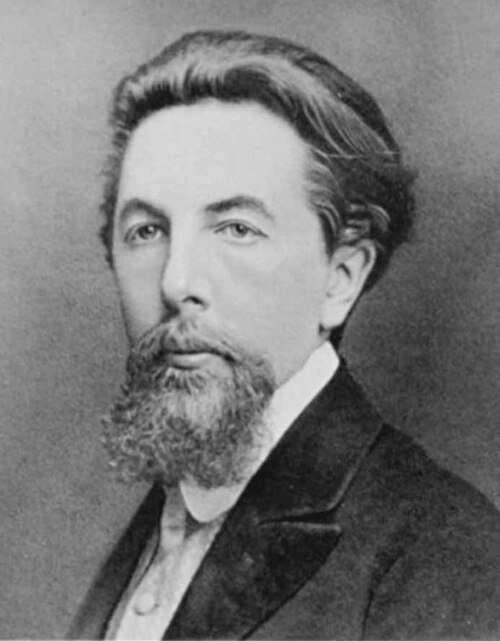
\includegraphics[width=\linewidth]{images/book3/tsvet.jpg}
\end{minipage}\hfill
\begin{minipage}[t]{0.78\linewidth}
\vspace{0pt}
El botánico Mijaíl Tsvet vertió un extracto de hojas verdes en un tubo de vidrio lleno de tiza
en polvo y lo hizo atravesar por un disolvente: los pigmentos se separaron en bandas coloreadas, clorofilas
verdes y carotenoides amarillos. En 1906 llamó al método \omterm{def:b2:chromatography:principle}{cromatografía}, ``escritura en colores''.
Fue en gran medida ignorado durante un cuarto de siglo, hasta que se retomó para los productos naturales en
los años treinta. (Retrato: autor desconocido, dominio público; Wikimedia Commons.)
\end{minipage}
\end{history}

\begin{safety}{\ghs[5mm]{GHS02}\,\ghs[5mm]{GHS05}\,\ghs[5mm]{GHS06}\,\ghs[5mm]{GHS07}\,\ghs[5mm]{GHS08}\,\ghs[5mm]{GHS09}}
El acetonitrilo y el metanol, los componentes orgánicos habituales de las \omterm{def:b2:chromatography:principle}{fases móviles} de HPLC, son inflamables y tóxicos;
el hexano, usado en \omterm{def:b2:chromatography:principle}{cromatografía} en columna, es inflamable, peligroso para la salud y tóxico para los organismos acuáticos.
Los residuos de disolventes se recogen y nunca se vierten por el desagüe.
% ledger: ghs:acetonitrile, ghs:methanol, ghs:hexane
\end{safety}

\section{Ejercicios}

\begin{exercise}[$\star$]\label{exo:b2:chromatography:1}
Un compuesto tiene $t_R = \qty{5.0}{min}$ en una columna cuyo \omterm{def:b2:chromatography:retention}{tiempo muerto} es \qty{1.0}{min}. Calcúlense su
\omterm{def:b2:chromatography:retention}{factor de retención} y la fracción de su tiempo que pasa en la \omterm{def:b2:chromatography:principle}{fase móvil}.
\end{exercise}

\begin{exercise}[$\star$]\label{exo:b2:chromatography:2}
Un pico con $t_R = \qty{6.0}{min}$ tiene una anchura en la base de \qty{0.30}{min}. Calcúlese el \omterm{def:b2:chromatography:plates}{número de platos}.
\end{exercise}

\begin{exercise}[$\star$]\label{exo:b2:chromatography:3}
Una columna de \qty{250}{mm} da $N = 10\,000$ para un compuesto. Calcúlese la \omterm{def:b2:chromatography:plates}{altura de plato}.
\end{exercise}

\begin{exercise}[$\star$]\label{exo:b2:chromatography:4}
¿CG o HPLC? Etanol en sangre; una proteína; cafeína en una bebida; benceno en gasolina; azúcares en un zumo de fruta.
\end{exercise}

\begin{exercise}[$\star\star$]\label{exo:b2:chromatography:5}
Dos picos: $t_{R1} = \qty{4.0}{min}$, $w_1 = \qty{0.40}{min}$; $t_{R2} = \qty{4.6}{min}$, $w_2 =
\qty{0.50}{min}$. Calcúlese la \omterm{def:b2:chromatography:separation}{resolución}. ¿Están separados hasta la línea de base?
\end{exercise}

\begin{exercise}[$\star\star$]\label{exo:b2:chromatography:6}
¿Cuántos platos se necesitan para separar dos compuestos con $\alpha = 1.10$ y $k_2 = 4.0$ con
$R_s = 1.5$?
\end{exercise}

\begin{exercise}[$\star\star$]\label{exo:b2:chromatography:7}
Una columna tiene $A = \qty{5}{\micro m}$, $B = \qty{8}{\micro m.mm/s}$, $C = \qty{2}{\micro m.s/mm}$
(datos de ejercicio). Hállense la velocidad óptima y la \omterm{def:b2:chromatography:plates}{altura de plato} mínima.
\end{exercise}

\begin{exercise}[$\star\star$]\label{exo:b2:chromatography:8}
Prevéase el orden de \omterm{def:b2:chromatography:principle}{elución} del benceno, el fenol y el tolueno en HPLC en \omterm{def:b2:chromatography:techniques}{fase inversa} con una
\omterm{def:b2:chromatography:principle}{fase móvil} agua--metanol, y qué ocurre cuando se aumenta la fracción de metanol.
\end{exercise}

\begin{exercise}[$\star\star$]\label{exo:b2:chromatography:9}
Una disolución de calibrado de un analito a \qty{20.0}{mg/L} con el \omterm{def:b2:chromatography:quantitative}{patrón interno} a \qty{10.0}{mg/L}
da áreas de 860 y 400. Una muestra a la que se añade el patrón a \qty{10.0}{mg/L} da áreas de 645 y 410.
Calcúlense el \omterm{def:b2:chromatography:quantitative}{factor de respuesta} y la concentración del analito (datos de ejercicio).
\end{exercise}

\begin{exercise}[$\star\star\star$]\label{exo:b2:chromatography:10}
Una separación da $R_s = 1.06$. ¿Qué longitud de columna, respecto a la actual, da $R_s = 1.5$, y
qué cuesta en tiempo? ¿Qué otras palancas hay?
\end{exercise}

\begin{exercise}[$\star\star\star$]\label{exo:b2:chromatography:11}
Para dos picos gaussianos de igual altura y anchura con anchura en la base $w = 4\sigma$, calcúlese la señal
en el punto medio entre ellos, relativa a la altura de pico, con $R_s = 1$ y con $R_s = 1.5$ (despréciese la contribución
del pico lejano en cada máximo).
\end{exercise}

\begin{exercise}[$\star\star\star$]\label{exo:b2:chromatography:12}
A $N$ y $\alpha$ constantes, compárense el factor de \omterm{def:b2:chromatography:separation}{resolución} $k_2/(1+k_2)$ y el tiempo de análisis relativo
$1 + k_2$ para $k_2 = 2$, 5 y 10. ¿Qué intervalo de $k$ se elegiría?
\end{exercise}

\section{Problema: la cafeína de una bebida energética}

\begin{problem}[{Problema de fin de semana --- el orden de elución en fase inversa, las prestaciones de la columna a partir de un
cromatograma, la mejora de la separación y la cuantificación con un patrón interno}]
\label{pb:b2:chromatography:1}
Datos de ejercicio (inventados, no se trata de un método real). Una bebida energética se diluye diez veces (de \qty{5.00}{mL} a
\qty{50.0}{mL}) y se añade teofilina como \omterm{def:b2:chromatography:quantitative}{patrón interno} a \qty{40.0}{mg/L} en la disolución
diluida. Columna: \qty{150}{mm}, \omterm{def:b2:chromatography:techniques}{fase inversa}; \omterm{def:b2:chromatography:principle}{fase móvil} agua--metanol; detección UV. La
matriz no retenida (azúcares y sales) eluye en $t_M = \qty{1.0}{min}$; la teofilina, a
\qty{3.0}{min} (anchura en la base \qty{0.18}{min}); la cafeína, a \qty{3.4}{min} (anchura en la base \qty{0.20}{min}).
Calibrado: cafeína a \qty{50.0}{mg/L} y teofilina a \qty{40.0}{mg/L} dan áreas de 1500 y 1000.
Muestra: áreas de 970 (cafeína) y 1010 (teofilina). Una lata contiene \qty{250}{mL}.
% ledger: ghs:caffeine, ghs:methanol

\begin{center}
\begin{tikzpicture}
\begin{axis}[width=0.75\linewidth, height=4.4cm, xmin=0, xmax=5, ymin=0, ymax=1,
  xlabel={tiempo (min)}, ylabel={absorbancia (u.a.)}, label style={font=\small},
  tick label style={font=\scriptsize}, ytick=\empty]
\addplot[omDef, thick] table[x=t, y=s] {figdata/out/bachelor-2-chromatogram-c.dat};
\node[font=\scriptsize] at (axis cs:1.0,0.42) {matriz};
\node[font=\scriptsize] at (axis cs:2.62,0.86) {teofilina};
\node[font=\scriptsize] at (axis cs:3.85,0.84) {cafeína};
\end{axis}
\end{tikzpicture}
\end{center}
% figdata: bachelor-2/chromatogram.py part c

\medskip
\noindent\textbf{Parte I --- \omterm{def:b2:chromatography:techniques}{Fase inversa}.}
\begin{enumerate}
  \item Descríbanse las \omterm{def:b2:chromatography:principle}{fases estacionaria} y móvil de una columna de \omterm{def:b2:chromatography:techniques}{fase inversa}.
  \item ¿Por qué los azúcares eluyen en el \omterm{def:b2:chromatography:retention}{tiempo muerto}?
  \item La cafeína es la 1,3,7-trimetilxantina, y la teofilina, la 1,3-dimetilxantina. Explíquese su orden de
        \omterm{def:b2:chromatography:principle}{elución}.
  \item ¿Por qué la teofilina es aquí un buen \omterm{def:b2:chromatography:quantitative}{patrón interno}?
  \item ¿Qué les ocurriría a ambos \omterm{def:b2:chromatography:retention}{tiempos de retención} si se aumentara la fracción de metanol?
  \item ¿Qué mide el \omterm{def:b2:chromatography:retention}{tiempo muerto}?
\end{enumerate}

\medskip
\noindent\textbf{Parte II --- Prestaciones de la columna.}
\begin{enumerate}[resume]
  \item Calcúlense los \omterm{def:b2:chromatography:retention}{factores de retención} de la teofilina y de la cafeína.
  \item Calcúlese el \omterm{def:b2:chromatography:separation}{factor de selectividad}.
  \item Calcúlese el \omterm{def:b2:chromatography:plates}{número de platos} para la cafeína y para la teofilina.
  \item Calcúlese la \omterm{def:b2:chromatography:plates}{altura de plato} para la cafeína.
  \item Calcúlese la \omterm{def:b2:chromatography:separation}{resolución} entre los dos picos.
  \item Compruébese con la ecuación de la \omterm{def:b2:chromatography:separation}{resolución}.
  \item ¿Están los picos separados hasta la línea de base?
\end{enumerate}

\medskip
\noindent\textbf{Parte III --- Más rápido o mejor.}
\begin{enumerate}[resume]
  \item Para ahorrar tiempo, se acorta la columna a \qty{75}{mm} (mismo relleno y mismo caudal). ¿Qué ocurre con
        la \omterm{def:b2:chromatography:separation}{resolución}?
  \item ¿Y con el tiempo de análisis?
  \item ¿Qué daría en cambio una columna de \qty{300}{mm}, y a qué coste?
  \item ¿Qué palanca actúa sobre $\alpha$?
  \item ¿Ayudaría mucho aquí aumentar $k$?
\end{enumerate}

\medskip
\noindent\textbf{Parte IV --- Cuantificación.}
\begin{enumerate}[resume]
  \item Calcúlese el \omterm{def:b2:chromatography:quantitative}{factor de respuesta} de la cafeína respecto a la teofilina.
  \item ¿Por qué no importa el volumen inyectado?
  \item Calcúlese la concentración de cafeína en la disolución diluida.
  \item Calcúlese la concentración de cafeína en la bebida.
  \item ¿Qué fallaría si un compuesto de la matriz coeluyera con la teofilina?
  \item ¿Qué exigiría en cambio un calibrado externo?
  \item Indíquese la masa de cafeína en una lata de \qty{250}{mL}.
\end{enumerate}
\end{problem}
